% \newcommand{\tedge}[5]{\draw[#3] (#1)-- node[e, #5] (e#4) {#4} (#2)}

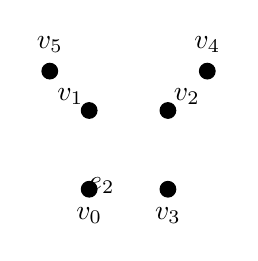
\begin{tikzpicture}
    \tikzstyle{v}=[draw, circle, minimum size=0.1cm, font=\footnotesize]
    \tikzstyle{c}=[draw, circle, inner sep=2, fill=black]
    \tikzstyle{e}=[]

    \node[c] (v0) at (  0,   0) [label=below:$v_0$]{};
    \node[c] (v1) at (  0,   1) [label={above left,inner sep=0pt,outer sep=0pt}:$v_1$]{};
    \node[c] (v2) at (  1,   1) [label={above right,inner sep=0pt,outer sep=0pt}:$v_2$]{};
    \node[c] (v3) at (  1,   0) [label=below:$v_3$]{};
    \node[c] (v4) at (1.5, 1.5) [label=above:$v_4$]{};
    \node[c] (v5) at (-.5, 1.5) [label=above:$v_5$]{};

    \tedge{v3}{v2}{solid}{}{};
    \tedge{v2}{v1}{solid}{}{};
    \tedge{v1}{v0}{solid}{}{};
    \tedge{v0}{v5}{solid}{}{};
    \tedge{v5}{v4}{solid}{}{};
    \tedge{v4}{v3}{solid}{}{};

    \tedge{v3}{v0}{solid}{}{};
    \tedge{v2}{v5}{dashed}{$e_2$}{above, pos=.35};
    \tedge{v1}{v4}{solid}{}{};
\end{tikzpicture}
